\documentclass[10pt,a4paper]{article}
\usepackage[latin1]{inputenc}
\usepackage{amsmath}
\usepackage{amsfonts}
\usepackage{amssymb}
\usepackage{fullpage}
\usepackage{graphicx}
\usepackage{parskip}
\usepackage{subcaption}

\begin{document}
\title{Thesis Work}
\author{Josh Orndorff \\ admin@joshorndorff.com}
\maketitle

\section{Definitions and Geometry}
\begin{figure}[htb]
\centering
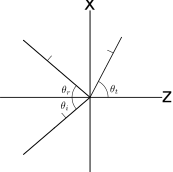
\includegraphics[scale=1.2]{diagrams/RayGeometryDiagramP.eps}
\caption{Geometry of the problem. Large arrows represent propagation direction of plane waves. Small arrows are direction of electric fields.}
\end{figure}

The medium on the left is home to the incident and reflected waves and has real refractive index, $n_1$.  The medium on the right is home to the transmitted wave and has complex refractive index, $\tilde{n}_2=n_2-i\gamma$. The gain factor is called $\gamma$, and the explicit negative sign in the definition means that positive gamma is gainy and negative gamma is lossy. All complex quantities will be explicitly indicated as such by the presence of a tilde over their variables. Having specified refractive indices as the fundamental quantities describing each medium, we can calculate their permittivities as $\epsilon_1=n_1^2$ and $\tilde{\epsilon}_2=\tilde{n}_2^2$.

The directions of the electric fields are shown.

As is standard, $\mathbf{k}$ vectors will point in the direction of propagation of their respective waves, and their magnitudes will be given by $k=n\frac{\omega}{c}$. This allows us to write the magnitudes of the three relevant wave numbers fairly straightforwardly.  Only $k_t$, for the transmitted wave, is at all non-obvious because of the gainy material.
\begin{equation}
\tilde{k}_t=\tilde{n}_2\frac{\omega}{c}
\end{equation}
\begin{equation}
\tilde{k}_t=(n_2-i\gamma)\frac{\omega}{c}
\end{equation}
If we define $k_t=n_2\frac{\omega}{c}$, the no-gain result, then we can write the three wave numbers as follows.
\begin{subequations}
\begin{equation}
k_i=k_r=n_1\frac{\omega}{c}
\end{equation}
\begin{equation}
\tilde{k}_t=k_t-i\gamma\frac{\omega}{c}
\end{equation}
\end{subequations}


\section{Wave functions and boundary conditions}
We want to write the explicit forms of each of the three waves in order to match boundary conditions and calculate the amplitude reflection coefficient.  Each wave can be written in the form \begin{equation}
\mathbf{E}_m(\mathbf{x},t)=\mathbf{E}_{0m}e^{i(\mathbf{k_m}\cdot\mathbf{x}-\omega t)}
\end{equation}
Here $\mathbf{E}_m$ does dot have a tilde despite the explicit $i$ in the exponent which indicates that the field is given by the real part of the expression alone.

As before we'll start with the transmitted wave because it is the most complex.
\begin{equation}
\mathbf{E}_t(\mathbf{x},t)=E_{0t}(\cos\theta_t\mathbf{\hat{x}}-\sin\theta_t\mathbf{\hat{z}})e^{i(\tilde{k}_{tx}x+\tilde{k}_{tz}z-\omega t)}
\end{equation}

Factoring $\frac{\omega}{c}$ out of the exponent gives
\begin{equation}
\mathbf{E}_t(\mathbf{x},t)=E_{0t}(\cos\theta_t\mathbf{\hat{x}}-\sin\theta_t\mathbf{\hat{z}})
e^{i\frac{\omega}{c}(\tilde{n}_2\sin\theta_tx+\tilde{n}_2\cos\theta_tz-ct)}
\end{equation}

Substituting the form of $\tilde{n}_2$
\begin{equation}
\mathbf{E}_t(\mathbf{x},t)=E_{0t}(\cos\theta_t\mathbf{\hat{x}}-\sin\theta_t\mathbf{\hat{z}})
e^{i\frac{\omega}{c}(n_2\sin\theta_tx-i\gamma\sin\theta_t x+n_2\cos\theta_tz-i\gamma \cos\theta_tz-ct)}
\end{equation}

Splitting the exponent into real and imaginary parts
\begin{equation}
\mathbf{E}_t(\mathbf{x},t)=E_{0t}(\cos\theta_t\mathbf{\hat{x}}-\sin\theta_t\mathbf{\hat{z}})
e^{i\frac{\omega}{c}(n_2\sin\theta_tx+n_2\cos\theta_tz-ct)}
e^{\gamma\frac{\omega}{c}(\sin\theta_tx+\cos\theta_tz)}
\end{equation}

Now we can write the first exponent back in terms of $k_t$, the no-gain wave number so that it looks similar to the other two wave forms.
\begin{subequations}\label{waveforms}
\begin{equation}
\mathbf{E}_i(\mathbf{x},t)=E_{0i}(\cos\theta_i\mathbf{\hat{x}}-\sin\theta_i\mathbf{\hat{z}})
e^{i(k_{ix}x+k_{iz}z-\omega t)}
\end{equation}
\begin{equation}
\mathbf{E}_r(\mathbf{x},t)=E_{0r}(\cos\theta_r\mathbf{\hat{x}}+\sin\theta_r\mathbf{\hat{z}})
e^{i(k_{rx}x+k_{rz}z-\omega t)}
\end{equation}
\begin{equation}\label{waveform-Et}
\mathbf{E}_t(\mathbf{x},t)=E_{0t}(\cos\theta_t\mathbf{\hat{x}}-\sin\theta_t\mathbf{\hat{z}})
e^{i(k_{tx}x+k_{tz}z-\omega t)}
e^{\gamma\frac{\omega}{c}(\sin\theta_tx+\cos\theta_tz)}
\end{equation}
\end{subequations}

The last exponential in the transmitted equation represents the growth that will occur in the transmitted wave because of the gain in medium two. Let's attempt to match the boundary conditions and see what results. Following the lead of JD Jackson, since we must meet the boundary conditions at all points on the $z=0$ plane at all times, the spacial and time variation of all fields must be equal in the plane. For non-gainy material this is simple, but the final exponential in Eq: \ref{waveform-Et} changes the situation slightly.  We will take the spacial and time dependence from Eqs: \ref{waveforms}.

\begin{equation}
k_{ix}x-\omega t =
k_{rx}x-\omega t =
k_{tx}x-\omega t +\frac{\gamma\omega}{ic}\sin(\theta_t)x
\end{equation}

It is clear that the time dependence is already satisfied (we can subtract $\omega t$ from each term).

\begin{equation}\label{boundary conditions}
k_{ix}x=
k_{rx}x=
k_{tx}x +\frac{\gamma\omega}{ic}\sin(\theta_t)x
\end{equation}

Investigating equality of the first two terms in Eq: \ref{boundary conditions} allows us to derive the law of reflection which is exactly the same is it would be for the non-gain case.
\begin{equation}
k_{ix}x=k_{rx}x
\end{equation}
\begin{equation}
n_1\frac{\omega}{c}\sin\theta_i x = n_1\frac{\omega}{c}\sin\theta_r x
\end{equation}
\begin{equation}
\theta_i=\theta_r
\end{equation}

Investigating the second two terms in Eq: \ref{boundary conditions} allows us to derive Snell's law, but, as I've mentioned, the gain factor makes our situation more complicated.
\begin{equation}
k_{rx}x=k_{tx}x +\frac{\gamma\omega}{ic}\sin(\theta_t)x
\end{equation}
\begin{equation}
n_1\frac{\omega}{c}\sin\theta_i x=n_2\frac{\omega}{c}\sin(\theta_t) x +\frac{\gamma\omega}{ic}\sin(\theta_t)x
\end{equation}
\begin{equation}\label{Snell's law expanded}
n_1\sin\theta_i=n_2\sin\theta_t -i\gamma\sin\theta_t
\end{equation}

This can be simplified further to
\begin{equation}\label{Snel's law standard}
n_1\sin\theta_i=\tilde{n}_2\sin\theta_t
\end{equation}

In some ways the expanded form is more illustrative, but the condensed form looks almost identical to the standard non-gainy equation. 

But we have an issue at hand.  The left side is real, and the right side appears to be properly complex (both real and imaginary parts non-zero). So how can we save the equation mathematically? There are a few options.
\begin{enumerate}
\item Conclude that light can only be incident at $\theta_i=\theta_t=0^\circ$.  This is of course not a valid physical constraint as I can shine a laser beam at a gain medium from any angle I like.
\item Let $\gamma=0$ at $z=0$ which is to say that there is no gain exactly at the boundary. I have a hard time with this logic as illustrated by the following thought experiment. Consider when medium 1 has a real index $n_1$ and medium two has a complex index $\tilde{n}_2=n_1-i\gamma$. That is to say that the two medium are exactly the same except that the second is gainy (or lossy). If the gain doesn't kick in right at the boundary, but rather some infinitesimal distance to the right, then we should be defining the boundary an infinitesimal distance to the right. Because the portion of medium two where the gain is not active, is exactly the same as medium one.
\item Introduce a complex value of $\tilde{\theta_t}=\theta_t +i \phi_t$. This solves the mathematical problem for sure, but what is the physical significance of a complex angle?  Is this really just a mathematically rigorous (or obfuscated depending on taste) way of saying the same thing as 2?
\end{enumerate}

\section{Deriving the amplitude reflection coefficient $r$}
In order to proceed to calculate $r$, we must choose one of the solutions that I proposed to save Snell's law and then proceed to match the actual boundary conditions at $z=0$.  I'll choose option number three ans let $\tilde{\theta_t}$ be complex.

\begin{subequations}\label{BCs}
\begin{equation}\label{E BC}
E_{ix}+E_{rx}=E_{tx}
\end{equation}
\begin{equation}\label{D BC}
D_{iz}+D_{rz}=D_{tz}
\end{equation}
\end{subequations}

We've already taken care of the spacial and time dependence of the waves and, as a result, found the law of reflection and Snell's law.  Now we just have to relate the waves' amplitudes which can be found in Eqs: \ref{waveforms}. We can rewrite the amplitudes eliminating all angles except for $\theta_i$ by using the following transformations.
\begin{subequations}\label{angle transformation}
\begin{equation}\label{theta_r transform}
\theta_r=\theta_i
\end{equation}
\begin{equation}\label{sin theta_t transform}
\sin\tilde{\theta_t}=\frac{n_1}{\tilde{n}_2}\sin\theta_i
\end{equation}
\begin{equation}\label{cos theta_t transform}
\cos\tilde{\theta_t}=\sqrt{1-\frac{n_1^2}{\tilde{n}_2^2}\sin^2\theta_i}
\end{equation}
\end{subequations}

Substituting these into the waveforms (Eq: \ref{waveforms}) we get the following amplitudes

\begin{subequations}\label{amplitudes}
\begin{equation}
\mathbf{E}_{0i}=E_{0i}(\cos\theta_i\mathbf{\hat{x}}-\sin\theta_i\mathbf{\hat{z}})
\end{equation}
\begin{equation}
\mathbf{E}_{0r}=E_{0r}(\cos\theta_i\mathbf{\hat{x}}+\sin\theta_i\mathbf{\hat{z}})
\end{equation}
\begin{equation}
\mathbf{E}_{0t}=E_{0t}(\sqrt{1-\frac{n_1^2}{\tilde{n}_2^2}\sin^2\theta_i}\mathbf{\hat{x}}-\frac{n_1}{\tilde{n}_2}\sin\theta_i\mathbf{\hat{z}})
\end{equation}
\end{subequations}

Substituting these waveforms into the parallel electric field continuity boundary condition (Eq: \ref{E BC}) we get
\begin{equation}
(E_{0i}+E_{0r})\cos\theta_i = E_{0t}\sqrt{1-\frac{n_1^2}{\tilde{n}_2^2}\sin^2\theta_i}
\end{equation}

Substituting the waveforms into the perpendicular displacement field continuity boundary condition (Eq: \ref{D BC}) we get
\begin{equation}
-n_1^2 E_{0i}\sin\theta_i+n_1^2E_{0r}\sin\theta_i = -\tilde{n}_2^2 E_{0t}\frac{n_1}{\tilde{n}_2}\sin\theta_i
\end{equation}
\begin{equation}
n_1(E_{0i}-E_{0r})=\tilde{n}_2E_{0t}
\end{equation}
\begin{equation}
E_{0t} = \frac{n_1}{\tilde{n}_2}(E_{0i}-E_{0r})
\end{equation}

Combining the two gives
\begin{equation}
(E_{0i}+E_{0r})\cos\theta_i=\frac{n_1}{\tilde{n}_2}(E_{0i}-E_{0r})\sqrt{1-\frac{n_1^2}{\tilde{n}_2^2}\sin^2\theta_i}
\end{equation}
\begin{equation}
E_{0i}\left(\cos\theta_i-\frac{n_1}{\tilde{n}_2}\sqrt{1-\frac{n_1^2}{\tilde{n}_2^2}\sin^2\theta_i}\right)=
-E_{0r}\left(\frac{n_1}{\tilde{n}_2}\sqrt{1-\frac{n_1^2}{\tilde{n}_2^2}\sin^2\theta_i}+\cos\theta_i\right)
\end{equation}
\begin{equation}\label{r}\boxed{
r=\frac{E_{0r}}{E_{0i}}=\frac
{n_1\sqrt{1-\frac{n_1^2}{\tilde{n}_2^2}\sin^2\theta_i}-\tilde{n}_2\cos\theta_i}
{n_1\sqrt{1-\frac{n_1^2}{\tilde{n}_2^2}\sin^2\theta_i}+\tilde{n}_2\cos\theta_i}
}\end{equation}

The form above is nice because it expresses the amplitude reflection coefficient, $r$, entirely in terms of input parameters to the problem. But the expression is fairly complicated it would be simpler if we had never used transformation Eq: \ref{cos theta_t transform}.
\begin{equation}\label{r(n,theta)}
r=\frac{n_1\cos\tilde{\theta}_t-\tilde{n}_2\cos\theta_i}
{n_1\cos\tilde{\theta}_t+\tilde{n}_2\cos\theta_i}
\end{equation}

It could also be put in terms of $\epsilon$'s and $k_z$'s if we multiply the top and bottom of the fraction by the quantity $n_1\tilde{n}_2\omega/c$.
\begin{equation}\label{r(k,e)}
r=\frac{\epsilon_1\tilde{k}_{tz}-\tilde{\epsilon}_2k_{iz}}{\epsilon_1\tilde{k}_{tz}+\tilde{\epsilon}_2k_{iz}}
\end{equation}

\subsection{Isolating Real and Imaginary Parts of $r$}
For most work, the form in Eq: \ref{r(k,e)} will be most useful, but it is also valuable to explicitly isolate the real and imaginary parts.  To help with the algebra, let me define

\begin{equation}
\left.
\begin{aligned}
a=\epsilon_1k_{tz}' \\
b=\epsilon_1k_{tz}'' \\
c=\epsilon_2'k_{iz} \\
d=\epsilon_2''k_{iz}
\end{aligned}
\right\}
\end{equation}

Such that.
\begin{equation}
r=\frac{a+ib-c-id}{a+ib+c+id}
\end{equation}

Separating explicitely,
\begin{equation}
r=\frac{(a-c)+i(b-d)}{(a+c)+i(b+d)}
\end{equation}

Multiplying by the bottom's conjugate,
\begin{equation}
r=\frac{[(a-c)+i(b-d)][(a+c)-i(b+d)]}{[(a+c)+i(b+d)][(a+c)-i(b+d)]}
\end{equation}
\begin{equation}
r=\frac{(a^2-c^2)-i(b+d)(a+c)+i(a+c)(b-d)+(b^2-d^2)}{(a+c)^2+(b+d)^2}
\end{equation}

Separating again,
\begin{equation}
r=\frac{a^2+b^2-c^2-d^2}{(a+c)^2+(b+d)^2}+i\frac{(a+c)(b-d)-(b+d)(a-c)}{(a+c)^2+(b+d)^2}
\end{equation}

Now we have to plug back in the meaningful values for a,b,c, and d. I'll do the real and imaginary parts separately.
\begin{equation}
\Re(r)=\frac{\epsilon_1^2k_{tz}'^2-\epsilon_2'^2k_{iz}^2+\epsilon_1^2k_{tz}''^2-\epsilon_2''^2k_{iz}^2}{(\epsilon_1k_{tz}'+\epsilon_2'k_{iz})^2+(\epsilon_1k_{tz}''+\epsilon_2''k_{iz})^2}
\end{equation}
\begin{equation}\boxed{
\Re(r)=\frac{\epsilon_1^2(k_{tz}'^2+k_{tz}''^2)-k_{iz}^2(\epsilon_2'^2+\epsilon_2''^2)}{(\epsilon_1k_{tz}'+\epsilon_2'k_{iz})^2+(\epsilon_1k_{tz}''+\epsilon_2''k_{iz})^2}
}\end{equation}

For the imaginary part,
\begin{equation}
\Im(r)=\frac{2(bc-ad)}{(a+c)^2+(b+d)^2}
\end{equation}
\begin{equation}
\Im(r)=\frac{2(\epsilon_1k_{tz}''\epsilon_2'k_{iz}-\epsilon_1k_{tz}'\epsilon_2''k_{iz})}{(\epsilon_1k_{tz}'+\epsilon_2'k_{iz})^2+(\epsilon_1k_{tz}''+\epsilon_2''k_{iz})^2}
\end{equation}
\begin{equation}\boxed{
\Im(r)=\frac{2\epsilon_1k_{iz}(k_{tz}''\epsilon_2'-k_{tz}'\epsilon_2'')}{(\epsilon_1k_{tz}'+\epsilon_2'k_{iz})^2+(\epsilon_1k_{tz}''+\epsilon_2''k_{iz})^2}
}\end{equation}


\section{Calculating the Reflectivity $R$ from $r$}
Our task now is to calculate the intensity reflection coefficient, $R$. Continuing from Eq: \ref{r(k,e)}, and letting, $\tilde{k}_{tz}=k'_{tz}+ik''_{tz}$, and $\tilde{\epsilon}_2=\epsilon'_2+i\epsilon''_2$.

\begin{equation}
r=\frac{
\epsilon_1(k'_{tz}+ik''_{tz})-(\epsilon'_2+i\epsilon''_2)k_{iz}
}{
\epsilon_1(k'_{tz}+ik''_{tz})+(\epsilon'_2+i\epsilon''_2)k_{iz}
}
\end{equation}

Explicitly separating real and imaginary parts,
\begin{equation}
r=\frac{
(\epsilon_1 k'_{tz}-\epsilon'_2k_{iz}) +i (\epsilon_1 k''_{tz}-\epsilon''_2k_{iz})
}{
(\epsilon_1 k'_{tz}+\epsilon'_2k_{iz}) +i (\epsilon_1 k''_{tz}+\epsilon''_2k_{iz})
}
\end{equation}

Recalling that $(a+ib)(a-ib)=a^2+b^2$, we can write
\begin{equation}
R=r^*r=\frac{
(\epsilon_1 k'_{tz}-\epsilon'_2 k_{iz})^2 + (\epsilon_1 k''_{tz}-\epsilon''_2 k_{iz})^2
}{
(\epsilon_1 k'_{tz}+\epsilon'_2 k_{iz})^2 + (\epsilon_1 k''_{tz}+\epsilon''_2 k_{iz})^2
}
\end{equation}

That's the expression, but we have yet to find explicit expressions for $\tilde{\epsilon}_2$ and $\tilde{k}_{tz}$.  It is easy to see from the definitions that
\begin{equation}
\left.
\begin{aligned}
\epsilon'&=n^2-\gamma^2 \\
\epsilon''&=-2n\gamma
\end{aligned}
\right\}
\end{equation}

Finding $\tilde{k}_{tz}$ isn't quite as easy.  In order to make the algebra a tiny bit simpler, I'll find $\tilde{p}_{tz} \equiv \tilde{k}_{tz}/k_0$. Let's start from the definition.
\begin{equation}
\tilde{p}_{tz}=\tilde{n}_2\cos\tilde{\theta}_t
\end{equation}

Using Eq: \ref{cos theta_t transform},
\begin{equation}
\tilde{p}_{tz}=\sqrt{\tilde{n}_2^2-n_1^2\sin^2\theta_i}
\end{equation}

And expanding the $\tilde{n}_2$,
\begin{equation}\label{p_tz-direct}
\tilde{p}_{tz}=\sqrt{n_2^2-\gamma^2-n_1^2\sin^2\theta_i-2in_2\gamma}
\end{equation}

From here we can square both sides and get a system of equations, or use the known results (for example see the ComplexSquareRoot.pdf document I found online).
\begin{equation}
p'^2_{tz}-p''^2_{tz}+2ip'_{tz}p''_{tz}=n_2^2-\gamma^2-n_1^2\sin^2\theta_i-2in_2\gamma
\end{equation}

Equating the real and imaginary parts gives the following system of two equations in two unknowns.
\begin{subequations}
\begin{equation}
p'^2_{tz}-p''^2_{tz}=n_2^2-\gamma^2-n_1^2\sin^2\theta_i
\end{equation}
\begin{equation}
p'_{tz}p''_{tz}=-n_2\gamma
\end{equation}
\end{subequations}

And substitution gives the following decoupled quartics for $p'_{tz}$ and $p''_{tz}$.
\begin{equation}\label{p_tz-system}
\left.
\begin{aligned}
p'^4_{tz}  - [n_2^2-\gamma^2-n_1^2\sin^2\theta_i]p'^2_{tz}  + n_2^2\gamma^2 = 0 \\
p''^4_{tz} + [n_2^2-\gamma^2-n_1^2\sin^2\theta_i]p''^2_{tz} - n_2^2\gamma^2 = 0
\end{aligned}
\right\}
\end{equation}

A few things are striking about this system of equations.
First since a quartic has multiple solutions, it looks like we'll have different quadrant options for $k_{tz}$ despite my specifying $n$ instead of $\epsilon$. I guess that problem was more fundamental than I expected.
Second, the equations are highly symmetric.
Third, solving these should tell us whether $\theta_t$ must be complex. If $\theta_t$ is real , then the definition $\tilde{p}_{tz}=\tilde{n}_2\cos\theta_t$ gives very simple results for $p'_{tz}$ and $p''_{tz}$.


\section{Different quadrants for $\tilde{k}_{tz}$ (or $\tilde{p}_{tz}$)}
We have established, via two different algebraic routes, that we will need to find expressions for the transmitted propagation vector's real and imaginary parts.  I prefer to work in terms of the dimensionless quantities $\tilde{p}_{tz}=\tilde{k}_{tz}/k_0$ to eliminate factors of $k_0$ in the equations (the fewer symbols floating around, the better in my opinion).

So let's find the solutions, visualize them in the complex plane, and discuss the physical significance of each.  Starting from either Eq: \ref{p_tz-direct} or Eq: \ref{p_tz-system} should give the same results. But, as we've discussed they are not unique. We need to complex number's square root.
\begin{equation}
p_{tz}'+ip_{tz}''=\sqrt{a+ib}
\end{equation}

In our case,
\begin{equation}
\left.
\begin{aligned}
a=n_2^2-\gamma^2-n_1^2\sin^2\theta_i \\
b=-2n_2\gamma \qquad
\end{aligned}
\right\}
\end{equation}

Or, using the $k$ and $\epsilon$ language,
\begin{equation}
\left.
\begin{aligned}
a=\epsilon_2'-\epsilon_1\sin^2\theta_i \\
b=\epsilon_2'' \qquad
\end{aligned}
\right\}
\end{equation}





\subsection{The fourth quadrant solution}
The fourth quadrant solution has a positive real part and negative imaginary part.

This solution's physical meaning is a right-traveling, growing-as-z-increases wave.

Fan claims this isn't possible beyond the critical angle because of arbitrarily high gain in the limit as $\gamma \to 0$. [TO DO] reread that section. wth is high gain as gamma -> 0??

Mansuripur claims this is possible beyond the critical angle because it is "universally" accepted below the critical angle, and there is no reason for the correct $\tilde{p}_{tz}$ choice to suddenly change at the critical angle.

\subsection{The second quadrant solution}
The second quadrant solution has a negative real part and positive imaginary part.

This solution's physical meaning is a left-traveling, growing-as-z-\emph{decreases} wave.

Fan claims this is possible.

Mansuripur claims this isn't possible because how would there be a left-traveling wave in medium two, AND why would the correct $\tilde{p}_{tz}$ solution suddenly change at the critical angle?


\section{Coordinate systems for Gaussian Beams}
list them

\section{Deriving the Discrete Fourier Transform}
In physics the Fourier transform is well established to be
\begin{equation}
F(k_x)=\int_{-\infty}^\infty E(x)e^{-ik_xx}\,\mathrm{d}x
\end{equation}

We want to sample the Electric field at a finite number of points across the beam. Using a field that is sampled in $x$ will yield a transformed field that is sampled in $k_x$. Naturally the integral then becomes a sum.
\begin{equation}
F_m(k_m)=\sum_{n=0}^{N-1} E_n(x_n)e^{-ik_mx_n}
\end{equation}

In the above, the exponentials, $e^{-ikx}$, are known as the transform's kernel.

$x_n = nL =$ the $n^{th}$ position sample (meters)

$k_m = mK =$ the $m^{th}$ wave number sample (radians per meter)

$L = 1/\kappa_s =$ the spacial sampling interval (meters)

$K = \kappa_s/N = 2\pi\kappa_s/N =$ wave number sampling interval (rad/meter)

I like to remember the analogy $k:\kappa::\omega:f$.

So finally combining all of the expressions above we can find the $m^{th}$ wave number sample to be
\begin{equation}
k_m=\frac{2\pi m}{LN}
\end{equation}

\appendix

\section{Further consideration on $\tilde{\theta_t}$}
We see now that $\tilde{\theta_t}$ must have indeed been complex by the following argument.  Consider if $\theta_t$ had indeed been real.

\begin{equation}
\tilde{p}_{tz} = \frac{\tilde{k}_{tz}}{k_0} = \tilde{n}_2\cos\theta_t
\end{equation}
\begin{equation}
\tilde{p}_{tz} = (n_2 - i\gamma) \cos\theta_t
\end{equation}
\begin{equation}
\left.
\begin{aligned}
p'_{tz}=n_2\cos\theta_t \\
p''_{tz}=-\gamma\cos\theta_t
\end{aligned}
\right\}
\end{equation}

We've seen that $\tilde{p}_{tz}$ is not simply proportional to $\tilde{n}_2$. Wait... right?  [TO DO] plot $p_{tz}$ vs $\cos]theta_t$. I guess use Eq: \ref{cos theta_t transform} with just the real part of $n_2$??


\section{Considerations on permittivity, $\epsilon$, versus refractive index, $n$}
I've chosen to use a material's refractive index $n$ as its fundamental property because given a refractive index, a permittivity can be uniquely calculated with $\epsilon=n^2$, whereas specifying $\epsilon$ allows two possibilities for $n$ and therefore does not uniquely specify the properties of the material.
I've shown in the previous section how, in complex index materials, the gain factor gamma causes a wave's amplitude to grow exponentially as the wave propagates through the gainy medium. I'll now derive a general expression for complex permittivity, $\tilde{\epsilon}=\epsilon'+i\epsilon''$ starting from complex refractive index.
\begin{equation}
\tilde{\epsilon}=\tilde{n}^2
\end{equation}
\begin{equation}
\tilde{\epsilon}=(n-i\gamma)^2
\end{equation}
\begin{equation}
\tilde{\epsilon}=n^2-2in\gamma-\gamma^2
\end{equation}
\begin{equation}
\tilde{\epsilon}=(n^2-\gamma^2)-i(2n\gamma)
\end{equation}
\begin{equation}
\left.
\begin{aligned}
\epsilon'&=n^2-\gamma^2 \\
\epsilon''&=-2n\gamma
\end{aligned}
\right\}
\end{equation}
So, we see that both the real and imaginary parts of the permittivity, $\tilde{\epsilon}$, depend on the gain factor, $\gamma$.

My previous understanding was that, like refractive index, the imaginary part of permittivity, $\epsilon''$ dealt with gain/loss and the real part, $\epsilon'$, dealt with propagation, but this appears not to be the case. Although, the signs of each part of $\epsilon$ are determined according to my original understanding.

Further, all of this has assumed non-magnetic materials where $\mu=1$. What if $\mu\neq1$?  Gainy materials clearly require complex refractive indices, but when we let $\epsilon\mu=\tilde{n}^2$ should the imaginary part come from $\epsilon$ or $\mu$ or both?

One consequence of all this is that we must define the critical angle as
\begin{equation}
\sin\theta_c = \sqrt{\frac{\epsilon_2'}{\epsilon_1}}=\sqrt{\frac{n_2^2-\gamma^2}{n_1^2}}
\end{equation}

Only in the special case of transparent materials, does this definition simplify to $\sin\theta_c=n_2/n_1$.

\end{document}